
This three-dimensional benchmark was first proposed by Busse et al (1993) \cite{bucc93}. 
It has been subsequently carried out in \cite{tack94,trha98,albe00,onmm06,dawk11,krhb12}.
We here focus on Case 1 of \cite{bucc93}:  an isoviscous bimodal convection experiment at $Ra=3\cdot 10^5$.

The domain is of size $a\times b\times h$ with $a=1.0079h$, $b=0.6283h$ with $h=2700$km. It is filled with a Newtonian fluid characterised by $\rho_0=3300{\rm kg}.{\rm m}^{-3}$, $\alpha=10^{-5}{\rm K}^{-1}$, 
$\mu=8.0198\times10^{23}{\rm Pa.s}$, 
$k=3.564{\rm W}.{\rm m}^{-1}.{\rm K}^{-1}$, 
$C_p=1080{\rm J}.{\rm K}^{-1}.{\rm kg}^{-1}$.
The gravity vector is set to ${\bm g}=(0,0,-10)^T$.
The temperature is imposed at the bottom  ($T=3700^\circ$C) and at the top ($T=0^\circ$C).

Note that using these numbers (as provided in the original paper), we arrive at Ra=29967.01, which 
is not exactly $3\cdot10^5$ as announced. Also, the heat diffusivity $\kappa=k/\rho_0 C_p$ is 
{\it exactly} $10^{-6}$.

The various measurements presented in \cite{bucc93} are listed hereafter:
\begin{itemize}
\item The Nusselt number $Nu$ computed at the top surface following Eq. (\ref{eqNu}):
\[
Nu = L_z \frac{\int\int_{z=L_z} \frac{\partial T}{\partial y} dx dy  }{\int \int_{z=0} T dx dy}
\]
\item the root mean square velocity $v_{rms}$ and the temperature mean square velocity $T_{rms}$
\item The vertical velocity $w$ and temperature $T$ at points ${\bm x}_1=(0,0,L_z/2)$, ${\bm x}_2=(L_x,0,L_z/2)$,
${\bm x}_3=(0,L_y,L_z/2)$ and ${\bm x}_4=(L_x,L_y,L_z/2)$;
\item the vertical component of the heat flux $Q$ at the top surface  at all four corners. 
\end{itemize}

\begin{center}
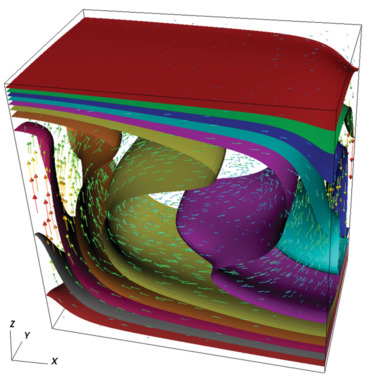
\includegraphics[width=5cm]{python_codes/fieldstone_20/images/krhb12}\\
{\captionfont Velocity field and isosurfaces of the temperature at steady state obtained 
with ASPECT.\\ Taken from Kronbichler et al (2012) \cite{krhb12}.}
\end{center}


\noindent Given the dimensions of the domain, here are resolutions that would yield (roughly) cubic elements:
\begin{center}
\begin{tabular}{l|lccccccc|}
1.0079$\times$2700km&nelx= &16 &20 &24 &28 &32 &36 &40 \\  
0.6283$\times$2700km&nely= &10 &13 &15 &18 &20 &23 &25 \\
1.0000$\times$2700km&nelz= &16 &20 &24 &28 &32 &36 &40 \\  
\end{tabular}
\end{center}

%............................
\subsubsection*{Methodology}

In what follows I highlight a few important points which are key to understanding how the code
is put together and works. 

\begin{verbatim}
load needed modules and functions
define parameters
build V grid (xV,yV,zV)
build V connectivity (iconV)
define b.c. for velocity (bc_fixV,bc_valV)
build T grid (xT,yT,zT)
build T connectivity (iconT)
define b.c. for temperature (bc_fixT,bc_valT)
initial temperature field
.------------------------> istep ---------------------.
|  build K,G,f,h                                      |
|  assemble them in A,rhs                             |
|  solve                                              |
|  split solution vector in u,v,w,p                   |
|  {u,v,w}=relax*{u,v,w}+(1-relax)*{u,v,w}            |
|  compute vrms                                       |
|  build A, rhs for temperature                       |
|  solve for temperature T                            |
|  T=relax*T+(1-relax)*T                              |
|  compute elemental strainrate                       |
|  compute nodal strainrate                           |
|  compute nodal pressure                             |
|  measure V and T at mid side edges, Nu ...          |
|  export to vtu and ascii files                      | 
.---------------------------<-------------------------.
\end{verbatim}

I fist load the shape functions which are in two separate files:

\begin{lstlisting}
from shape_functionsV import NNV,dNNVdr,dNNVds,dNNVdt
from shape_functionsT import NNT,dNNTdr,dNNTds,dNNTdt
\end{lstlisting}

There are NV=nnx*nny*nnz velocity nodes and NT=NV temperature nodes.

The velocity grid is built: xV, yV, zV, iconV, and 
these are copied in xT, yT, zT and iconT for the temperature grid.  

The initial temperature field is built as follows:
\begin{lstlisting}
for i in range(0,NT):
   T[i]= (Temperature2-Temperature1)/Lz*zT[i]+Temperature1 \
       + 100*(np.cos(np.pi*xT[i]/Lx) + np.cos(np.pi*yT[i]/Ly))*np.sin(np.pi*zT[i]/Lz)
\end{lstlisting}

The ${\bm C}$ matrix of Eq.~\ref{eq:mixedC} is then built:
\begin{lstlisting}
c_mat = np.array([[2,0,0,0,0,0],\
                  [0,2,0,0,0,0],\
                  [0,0,2,0,0,0],\
                  [0,0,0,1,0,0],\
                  [0,0,0,0,1,0],\
                  [0,0,0,0,0,1]],dtype=np.float64) 
\end{lstlisting}


\paragraph{Getting to steady state}  
In this case we are not so much interested in the path to steady state since 
the published values/measurements are {\it at} steady state.
The mass and momentum conservation equations for incompressible Stokes flow do not 
contain a time derivative but the energy conservation equation does. 
At steady state the terms $\partial_t T$ is zero by definition so we must solve
the following equation\footnote{Adiabtic heating, shear heating and internal heating are not considered
in the benchmark} (see Section~\ref{ss:hte}):
\begin{equation}
\vec{\upnu}\cdot\vec\nabla T - {\vec \nabla} \cdot k {\vec \nabla} T = 0
\end{equation}
The Finite Element discretisation of this equation yields 
\[
({\bm K}_a + {\bm K}_d) \cdot \vec{T} = \vec{0}
\]
which is much simpler than the time-dependent one and avoids to carefully consider the 
time-discretisation altogether. 

We now have to solve three coupled equations:
\begin{eqnarray}
-{\vec \nabla}p + {\vec \nabla}\cdot (2 \eta \dot{\bm \varepsilon}^d ) + \rho(T) {\vec g} &=& \vec{0} \\
{\vec \nabla}\cdot{\vec \upnu} &=& 0 \\ 
\vec{\upnu}\cdot\vec\nabla T - {\vec \nabla} \cdot k {\vec \nabla} T &=& 0 
\end{eqnarray}
We could then proceed to write the weak forms of these equations and cast these as we have done before, 
but this time considering velocity, pressure and temperature as unknowns of a (very) large system:
\[
\left(
\begin{array}{ccc}
\K & \G & . \\
\G^T & 0 & . \\
. & . & . 
\end{array}
\right)
\cdot
\left(
\begin{array}{c}
V \\ P \\ T 
\end{array}
\right)
=
\left(
\begin{array}{c}
. \\ . \\ .
\end{array}
\right)
\]
Once this matrix is filled a single solve will yield the steady state velocity, pressure and 
temperature fields! 

The term $\rho(T)$ will naturally end up in the (1,3) block of the assembled matrix as matrix ${\bm L}$.
The mass conservation equation in thisform is independent of temperature so the (2,3) block 
will be zero. The diffusion term ${\bm K}_d$ naturally finds its way to the (3,3) 
block and since there is not occurence of pressure in the energy equation the (3,2) 
block will be zero. We then obtain:
\[
\left(
\begin{array}{ccc}
\K & \G & {\bm L} \\
\G^T & 0 & 0 \\
. & 0 & {\bm K}_d 
\end{array}
\right)
\cdot
\left(
\begin{array}{c}
V \\ P \\ T 
\end{array}
\right)
=
\left(
\begin{array}{c}
. \\ . \\ .
\end{array}
\right)
\]
The last remaining term is the advection term of the energy equation and it is a problematic one:
it features the product of the velocity by the temperature. As such it is nonlinear and one cannot 
either put it in the (3,1) block nor in the (3,3) block. 

This approach fails, which is why 
the problem is solved iteratively. The idea is simple: when solving the 
coupled mass and momentum equations, assume temperature known, and when solving the energy equation
assume velocity known. We can then alternatively solve one system and then the other, constantly 
updating the fields when re-building the matrices or right hand sides.

However, it is well known that a straightforward implementation of this algorithm does not 
work in practice, i.e. it fails to converge, which is why a relaxation scheme is often implemented.
\begin{enumerate}
\item Solve for velocity and pressure
\item relax velocity
\begin{lstlisting}
u=relax*u+(1-relax)*u_old
v=relax*v+(1-relax)*v_old
w=relax*w+(1-relax)*w_old
\end{lstlisting}
\item Solve for temperature
\item relax temperature
\begin{lstlisting}
T=relax*T+(1-relax)*T_old
\end{lstlisting}
\item check for convergence:
\begin{lstlisting}
if np.abs(Nu-Nu_old)<1.e-5:
   break
\end{lstlisting}
\item store old fields
\begin{lstlisting}
u_old=u
v_old=v
w_old=w
T_old=T
\end{lstlisting}
\end{enumerate}

\paragraph{Computing nodal derivatives}  
Another interesting approach here is how the strain rate is computed on the nodes as well as
the temperature gradient. The strain rate is not needed for the required measurements of this 
benchmark but the Nusselt number calculations require $\partial T/\partial z$ at the top
boundary.    
The idea is simple: loop over all elements, and for each element loop over its support nodes
(in this case the 2x2x2 nodes of the $Q_1$), compute the required derivative there and add its contribution 
to the nodal field. Finally divide the obtained field by the number of elements each node is 
part of.




\newpage
%.......................
\subsubsection*{Results}

Given how the code is written and how costly second order elements are, high resolution
runs take a {\it very} long time to run, even using relaxation instead of time stepping. 

\begin{center}
%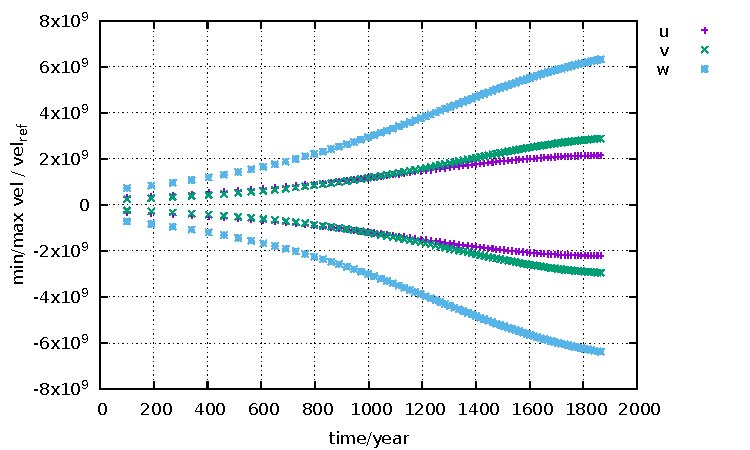
\includegraphics[width=7cm]{python_codes/fieldstone_20/results/velstats.pdf}
%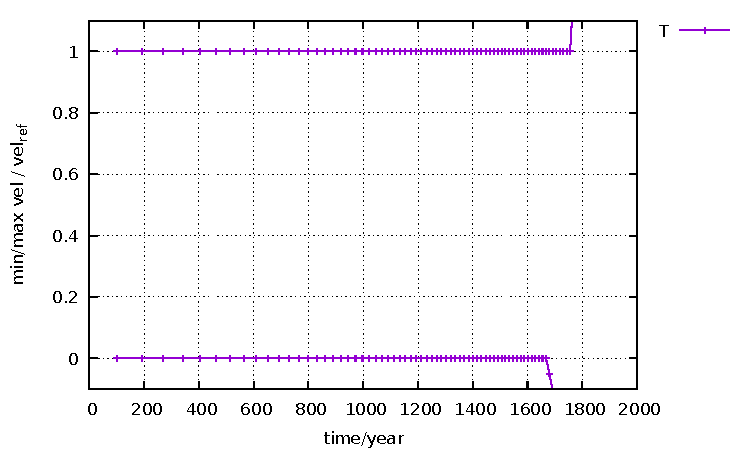
\includegraphics[width=7cm]{python_codes/fieldstone_20/results/Tstats.pdf}
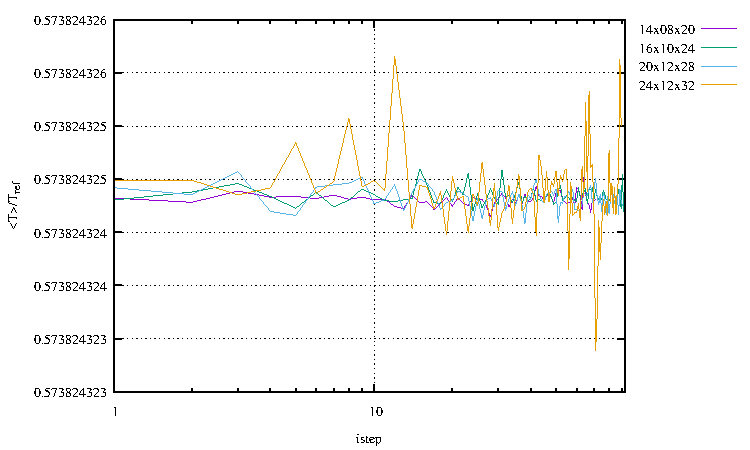
\includegraphics[width=7.5cm]{python_codes/fieldstone_20/results/Tavrg.pdf}\\
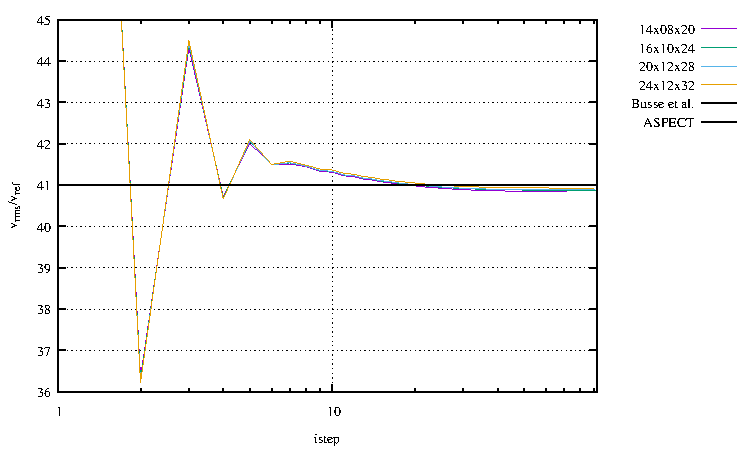
\includegraphics[width=7.5cm]{python_codes/fieldstone_20/results/vrms.pdf}
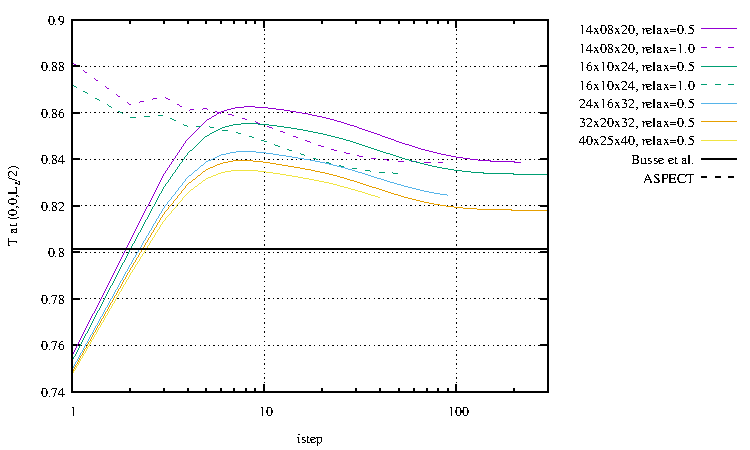
\includegraphics[width=7.5cm]{python_codes/fieldstone_20/results/Tmid.pdf}\\
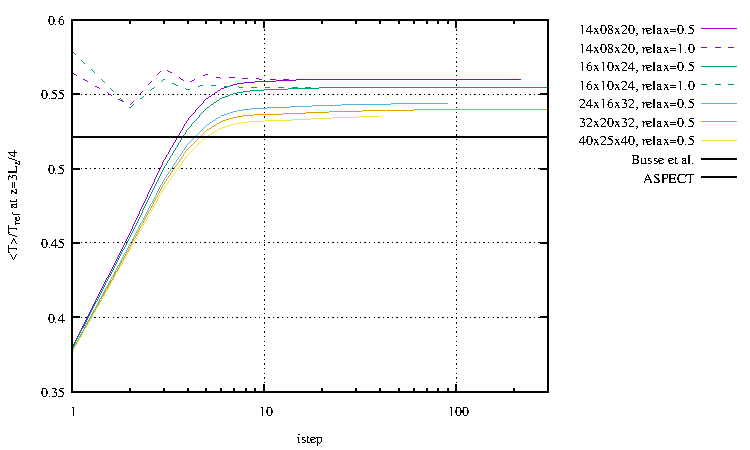
\includegraphics[width=7.5cm]{python_codes/fieldstone_20/results/Tm.pdf}
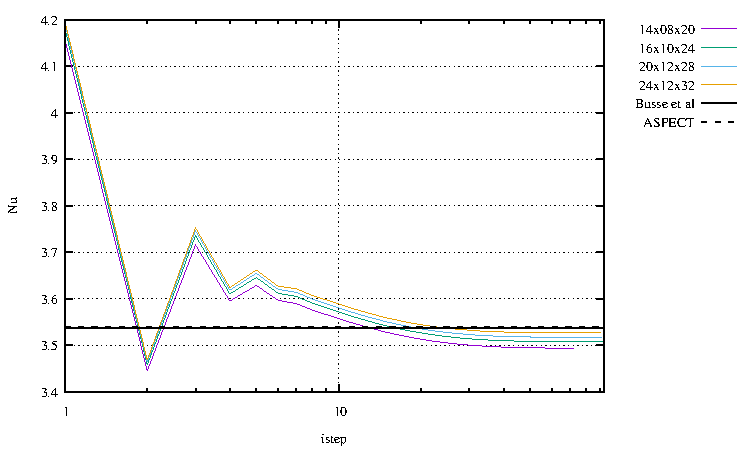
\includegraphics[width=7.5cm]{python_codes/fieldstone_20/results/Nu.pdf}\\
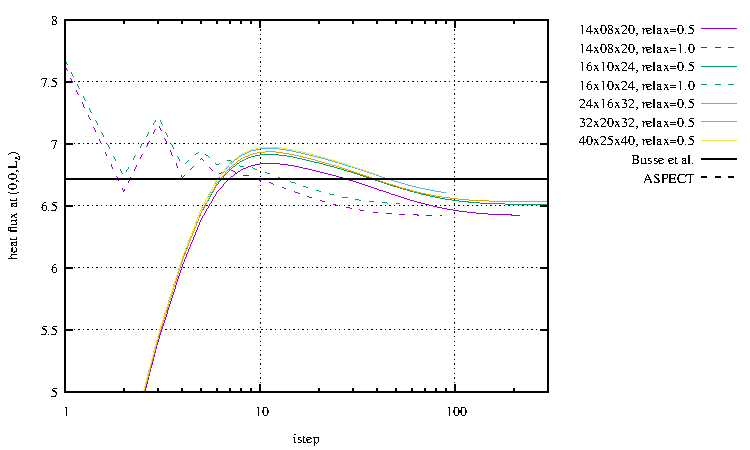
\includegraphics[width=7.5cm]{python_codes/fieldstone_20/results/hf1.pdf}
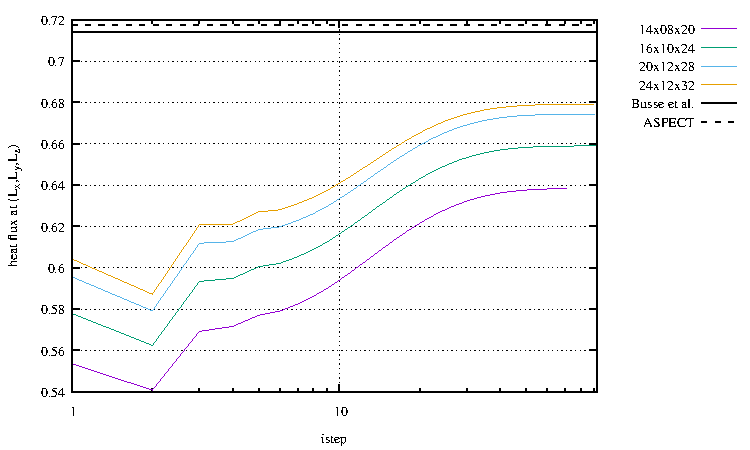
\includegraphics[width=7.5cm]{python_codes/fieldstone_20/results/hf2.pdf}\\
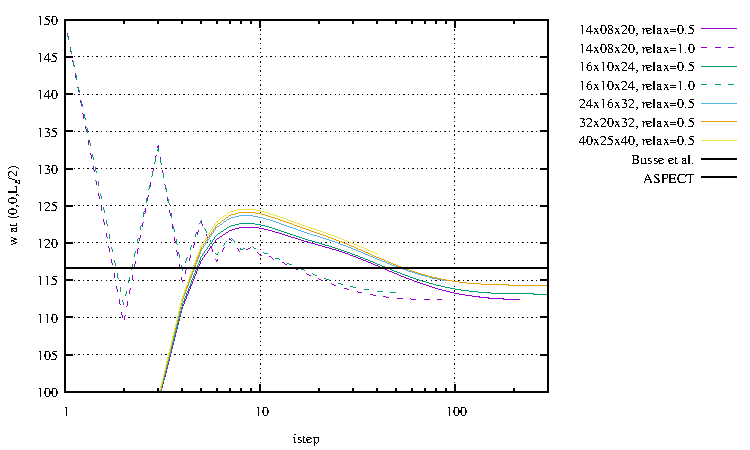
\includegraphics[width=7.5cm]{python_codes/fieldstone_20/results/wmid1.pdf}
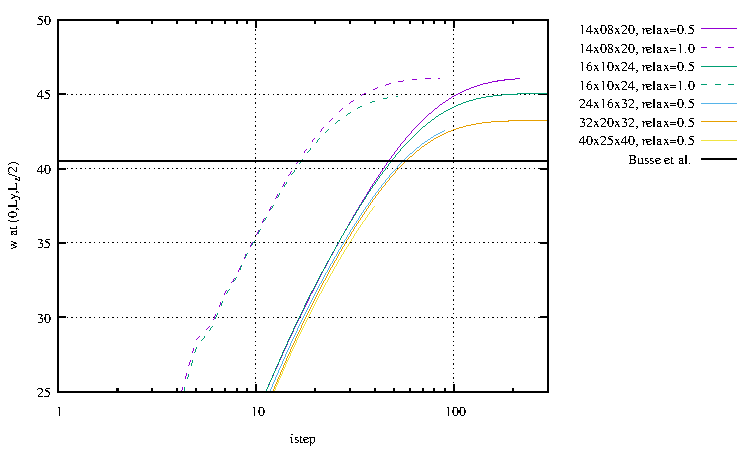
\includegraphics[width=7.5cm]{python_codes/fieldstone_20/results/wmid2.pdf}
\end{center}

The reported values for Busse et al. in the following table are taken from Table 3 of \cite{bucc93}.
The reported values for fieldstone are adimensionalised by means of a reference temperature (3700K),
a reference lengthscale 2700km, and a reference time $L_z^2/\kappa\sim 7.29e+18$s.
%The steady state is arrived at by solving the steady state Stokes and temperature equations 
%with a relaxation parameter of 1/2.
%To find the steady state, we simulate the problem up to non-dimensional time $t=5$, 
%i.e. $t=3.645e+19$s.



\begin{tabular}{llllll}
\hline
                                & ASPECT & ($Q_2\times Q_1/Q_1$)      &       & Busse et al \cite{bucc93} &  \\
Mesh size                       & Lz/24  & Lz/32 & Lz/48 & (best results)            & \\ 
\hline
Nu                              & 3.5539 &3.5447 & 3.5397 & $3.5374  \pm 0.0005$   \\
$v_{rms}$                       & 40.997 &40.999 &40.999  & $40.999  \pm 0.004$    \\
$\langle T\rangle$ at $0.75*Lz$ & 0.52148 & 0.52148&0.52148  & $0.52148 \pm 0.00003$  \\
$w(0,0,L_z/2)$     & 116.605 & 116.618 &  116.623  & $116.625 \pm 0.030$ \\
$w(L_x,0,L_z/2)$   & - &-&-& -\\
$w(L_x,L_y,L_z/2)$ & - &-&-& -\\
$w(0,L_y,L_z/2)$   &  &&& $40.500 \pm 0.030$ \\

$T(0,0,L_z/2)$     &  0.80126 & 0.80128 & 0.80129 & $0.80130 \pm 0.00005$ \\
$T(L_x,0,L_z/2)$   &  -&-&-& -\\
$T(L_x,L_y,L_z/2)$ &  -&-&-& -\\
$T(0,L_y,L_z/2)$   &  &&& $0.61876 \pm 0.00005$ \\
$dTdz(0,0,L_z)$    & 6.7679 & 6.7357 & 6.7189 & $6.7127 \pm 0.0500$ \\
$dTdz(L_x,0,L_z)$  &  & & & $1.5080 \pm 0.0500$ \\
$dTdz(L_x,L_y,L_z)$& 0.7237 & 0.7205 & 0.7174 & $0.7140 \pm 0.0500$ \\
$dTdz(0,L_y,L_z)$  &  & & & $3.1740 \pm 0.0500$ \\
\hline
\end{tabular}

\vspace{1cm}

THIS IS NOT FINISHED: I need to run the model at higher resolutions, which will take a few days.

